\documentclass{beamer}
\setbeamertemplate{footline}[frame number]
\usepackage{xcolor}
\usepackage{hyperref}
\usepackage{tikz}
\usepackage{graphicx}
\usepackage{xepersian}
\settextfont{XB Niloofar}
%%%%%%%%%%%%%%%%%%55
%%%%%%%%%%%%%%%%%%%%55
%%%%%%%%%%%%%%%%%%%%%%%
\begin{document}
\title{کمک گرفتن از \LaTeX~برای ارائه‌ی شفاهی}
\subtitle{درس شیوه‌ی ارائه‌ی مطالب علمی و فنّی}
\author{پوریا چراغی \\ \texttt{p.cheraaghi@gmail.com}}
\institute{دانشگاه گیلان}
%%%%%%%%%%%%%%%%%%
\begin{frame}
	\titlepage
\end{frame}
%%%%%%%%%%%%%%%%%%
%
%
\section{نفس ارائه‌ی شفاهی}
%
%
%%%%%%%%%%%%%%%%%%
\begin{frame}[t]{نکاتی درباره‌ی ارائه‌ی شفاهی}
\begin{itemize}
	\item<2->{حضور کامل فیزیکی مخاطب}
		\only<3>{\newline حواسّ بیشتر \tikz \draw[-stealth] (0,0) -- (-2,0); \textcolor[rgb]{0,0.5,0}{راه‌های ورود اطّلاعات بیشتر}}
	\item<4->{استفاده‌ی هوشمندانه از ابزار موجود}
		\only<5>{\newline حواسّ بیشتر \tikz \draw[-stealth] (0,0) -- (-2,0); \textcolor[rgb]{1,0,0}{راه‌های حواس‌پرتیِ بیشتر}}
	\item<6->{هنجارها}
		\only<7-10>{\newline راه تماس با ارائه‌کننده}
		\only<8-10>{\newline شماره‌بندیِ عناصر بصری}
		\only<9>{\newline \textcolor{red}{تمرین:} این هنجارها را در فصلِ ۹ از \cite{shahbahrami} و فصلِ ۴ از \cite{rankoohi} مرور کنید. (هدف این است که آمادگیِ ذهنی برای رعایتِ این نکات را- در صورت نیاز- داشته باشید.) 
\begin{tikzpicture} \draw[red, very thick] (0,0)--(0.25, 0.5)--(0.5,0)--cycle; \draw[red] (0.25, 0.35)--(0.25, 0.15); \draw[red] (0.25, 0.10) -- (0.25, 0.05); \end{tikzpicture} حینِ مطالعه‌ی این فصل‌ها، خطاهای نگارشی و دستوری را- که به چشم‌تان می‌آید- گزارش کنید.}
	\item<11->{}
\end{itemize}
\end{frame}
%%%%%%%%%%%%%%%%%%%
%
%
\section{استفاده از \LaTeX}
%
%
%%%%%%%%%%%%%%%%
\begin{frame}[t]
	\frametitle{ارائه با \LaTeX}
	\framesubtitle{کلاسِ \lr{\texttt{beamer}}}
	\begin{itemize}
		\item \only<2-6>{رعایت شدن هنجارهای رایج به صورت خودکار}
		\item \only<3-6>{آماده‌سازی ارائه‌ی قابل قبول در زمان کوتاه}
	\end{itemize}
	\only<4>{\textcolor{red}{تمرین:} با دستور \lr{\scriptsize \texttt{user@linuxmachine -\$ texdoc beamer}}، \href{https://mirror.bardia.tech/ctan/macros/latex/contrib/beamer/doc/beameruserguide.pdf}{\textcolor{blue}{\underline{راهنمای کاربریِ \lr{\texttt{beamer}}}}} را باز کرده، نگاهی به قسمت‌های مختلف آن بیندازید.}
	\only<5>{\textcolor{red}{تمرین:} از \lr{\texttt{\textbackslash tableofcontents}} استفاده کنید و یک صفحه با عنوان دورنما، بعد از صفحه‌ی عنوان، بسازید.}
\end{frame}
%%%%%%%%%%%%%%%%
%%%%%%%%%%%%%%%%%
\begin{frame}[t]
	\frametitle{اهمّیّت شکل‌ها}
	\framesubtitle{نقّاشی با~\LaTeX}
	\only<2-9>{استفاده از بسته‌ی \lr{\texttt{tikz}}}
	\only<3>{\newline \flushleft \scriptsize \lr{\texttt{\textbackslash begin\{tikzpicture\}\textbackslash draw (0,0)--(1,2);\textbackslash end\{tikzpicture\}}}}
	\only<3>{\newline \newline \newline \newline \newline \newline \newline \newline \begin{tikzpicture} \draw (0,0)--(0.5,1); \end{tikzpicture}}
	\only<4>{\newline \flushleft \scriptsize \lr{\texttt{\textbackslash begin\{tikzpicture\}\textbackslash draw (0,0)--(1,2)--(2,0);\textbackslash end\{tikzpicture\}}}}
	\only<4>{\newline \newline \newline \newline \newline \newline \newline \newline 
\begin{tikzpicture} \draw (0,0)--(0.5,1)--(1,0); \end{tikzpicture}}
	\only<5>{\newline \flushleft \scriptsize \lr{\texttt{\textbackslash begin\{tikzpicture\}\textbackslash draw (0,0)--(1,2)--(2,0)--cycle;\textbackslash end\{tikzpicture\}}}}
	\only<5>{\newline \newline \newline \newline \newline \newline \newline \newline 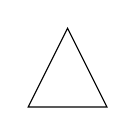
\begin{tikzpicture} \draw (0,0)--(0.5,1)--(1,0)--cycle; \end{tikzpicture}}
	\only<6>{\newline \textcolor{red}{تمرین:} از دستورِ \newline \lr{\texttt{user@linuxmachine -\$ texdoc tikz}} \newline استفاده کنید، تا با توجه به \href{https://mirrors.mi-ras.ru/CTAN/graphics/pgf/base/doc/pgfmanual.pdf}{\textcolor{blue}{\underline{راهنمای کاربریِِ \lr{\texttt{tikz}}}}}، کدِ مناسب برای نوشتن طول اضلاع کنارِ آن‌ها را بیابید.}
	\only<6>{\newline \begin{center}\includegraphics[trim=9cm 24.5cm 9cm 3.5cm, clip, width=5cm]{fig.pdf}\end{center}}
	\only<7>{\newline با استفاده از \lr{\texttt{\textbackslash geometry\{a4paper\}}} از یکسان بودن اندازه‌ها در نسخه‌ی چاپی مطمئن شوید.}
	\only<8>{\newline \textcolor{red}{تمرین:} \href{./seminar.pdf}{شعر «سمینار»} را با بسته‌ی \lr{\texttt{\textbackslash bidipoem}} حروف‌چینی کنید.}
\end{frame}
%
%
%%%%%%%%%%%%%%%%%%%
\begin{frame}
	\frametitle{واژه‌نامه}
	\framesubtitle{معادل فارسی برای واژه‌های بیگانه‌ای که استفاده کردم}
	\begin{center}
		\scriptsize
		\begin{tabular}{l|r}
			واژه‌ی بیگانه&معادل فارسی\\
			\hline
			label&\textcolor{red}{برچسب}\\
			documentation&مستند‌سازی\\
			caption&عنوان\\
			typeset&حروف‌چینی کردن\\
			font&قلم\\
			interface&رابط\\
			edit&ویرایش کردن\\
		\end{tabular}
	\end{center}
\end{frame}
%%%%%%%%%%%%%%%%%%
\section{مراجع}
%%%%%%%%%%%%%
\begin{frame}
	\frametitle{مراجع}
\bibliographystyle{plainnat-fa}
\bibliography{ref}
\end{frame}
%
%


\end{document}
